\documentclass{article}

\usepackage[utf8]{inputenc}
\usepackage[T1]{fontenc}
\usepackage[francais]{babel}
\usepackage[top = 1.5cm, left = 1.5cm, right =1.5cm, bottom = 1.5cm]{geometry}
\usepackage[pdfborder ={0 0 0}]{hyperref}
\usepackage{graphicx}
\usepackage{xcolor}
\usepackage{multicol}
\usepackage{lscape}
\usepackage{datatool}
\usepackage{pdfpages}
\usepackage{rotating}
\usepackage{xspace}
\usepackage{titlesec}
\usepackage{roboto}

\definecolor{title-color}{gray}{0.30}

\setlength{\parindent}{15pt}
\setlength{\parskip}{5pt}

\titleformat{\section}
  {\clearpage\normalfont\sffamily\Huge\bfseries\centering\robotoslab\color{title-color}}
  {}{0pt}{\bigskip}

\titleformat{\subsection}
  {\normalfont\sffamily\LARGE\bfseries\robotoslab\color{title-color}}
  {\thesubsection}{1em}{}

\begin{document}

\begin{titlepage}
\begin{figure}
\end{figure}

\title{\vspace{1cm}{\Huge \bf{\color{title-color}\robotoslab Management Project} } \\ \vspace{2cm} \bf{\color{title-color}\robotoslab Mold \& Co in China} \vspace{1cm} \\
}
\begin{figure}
\begin{center}
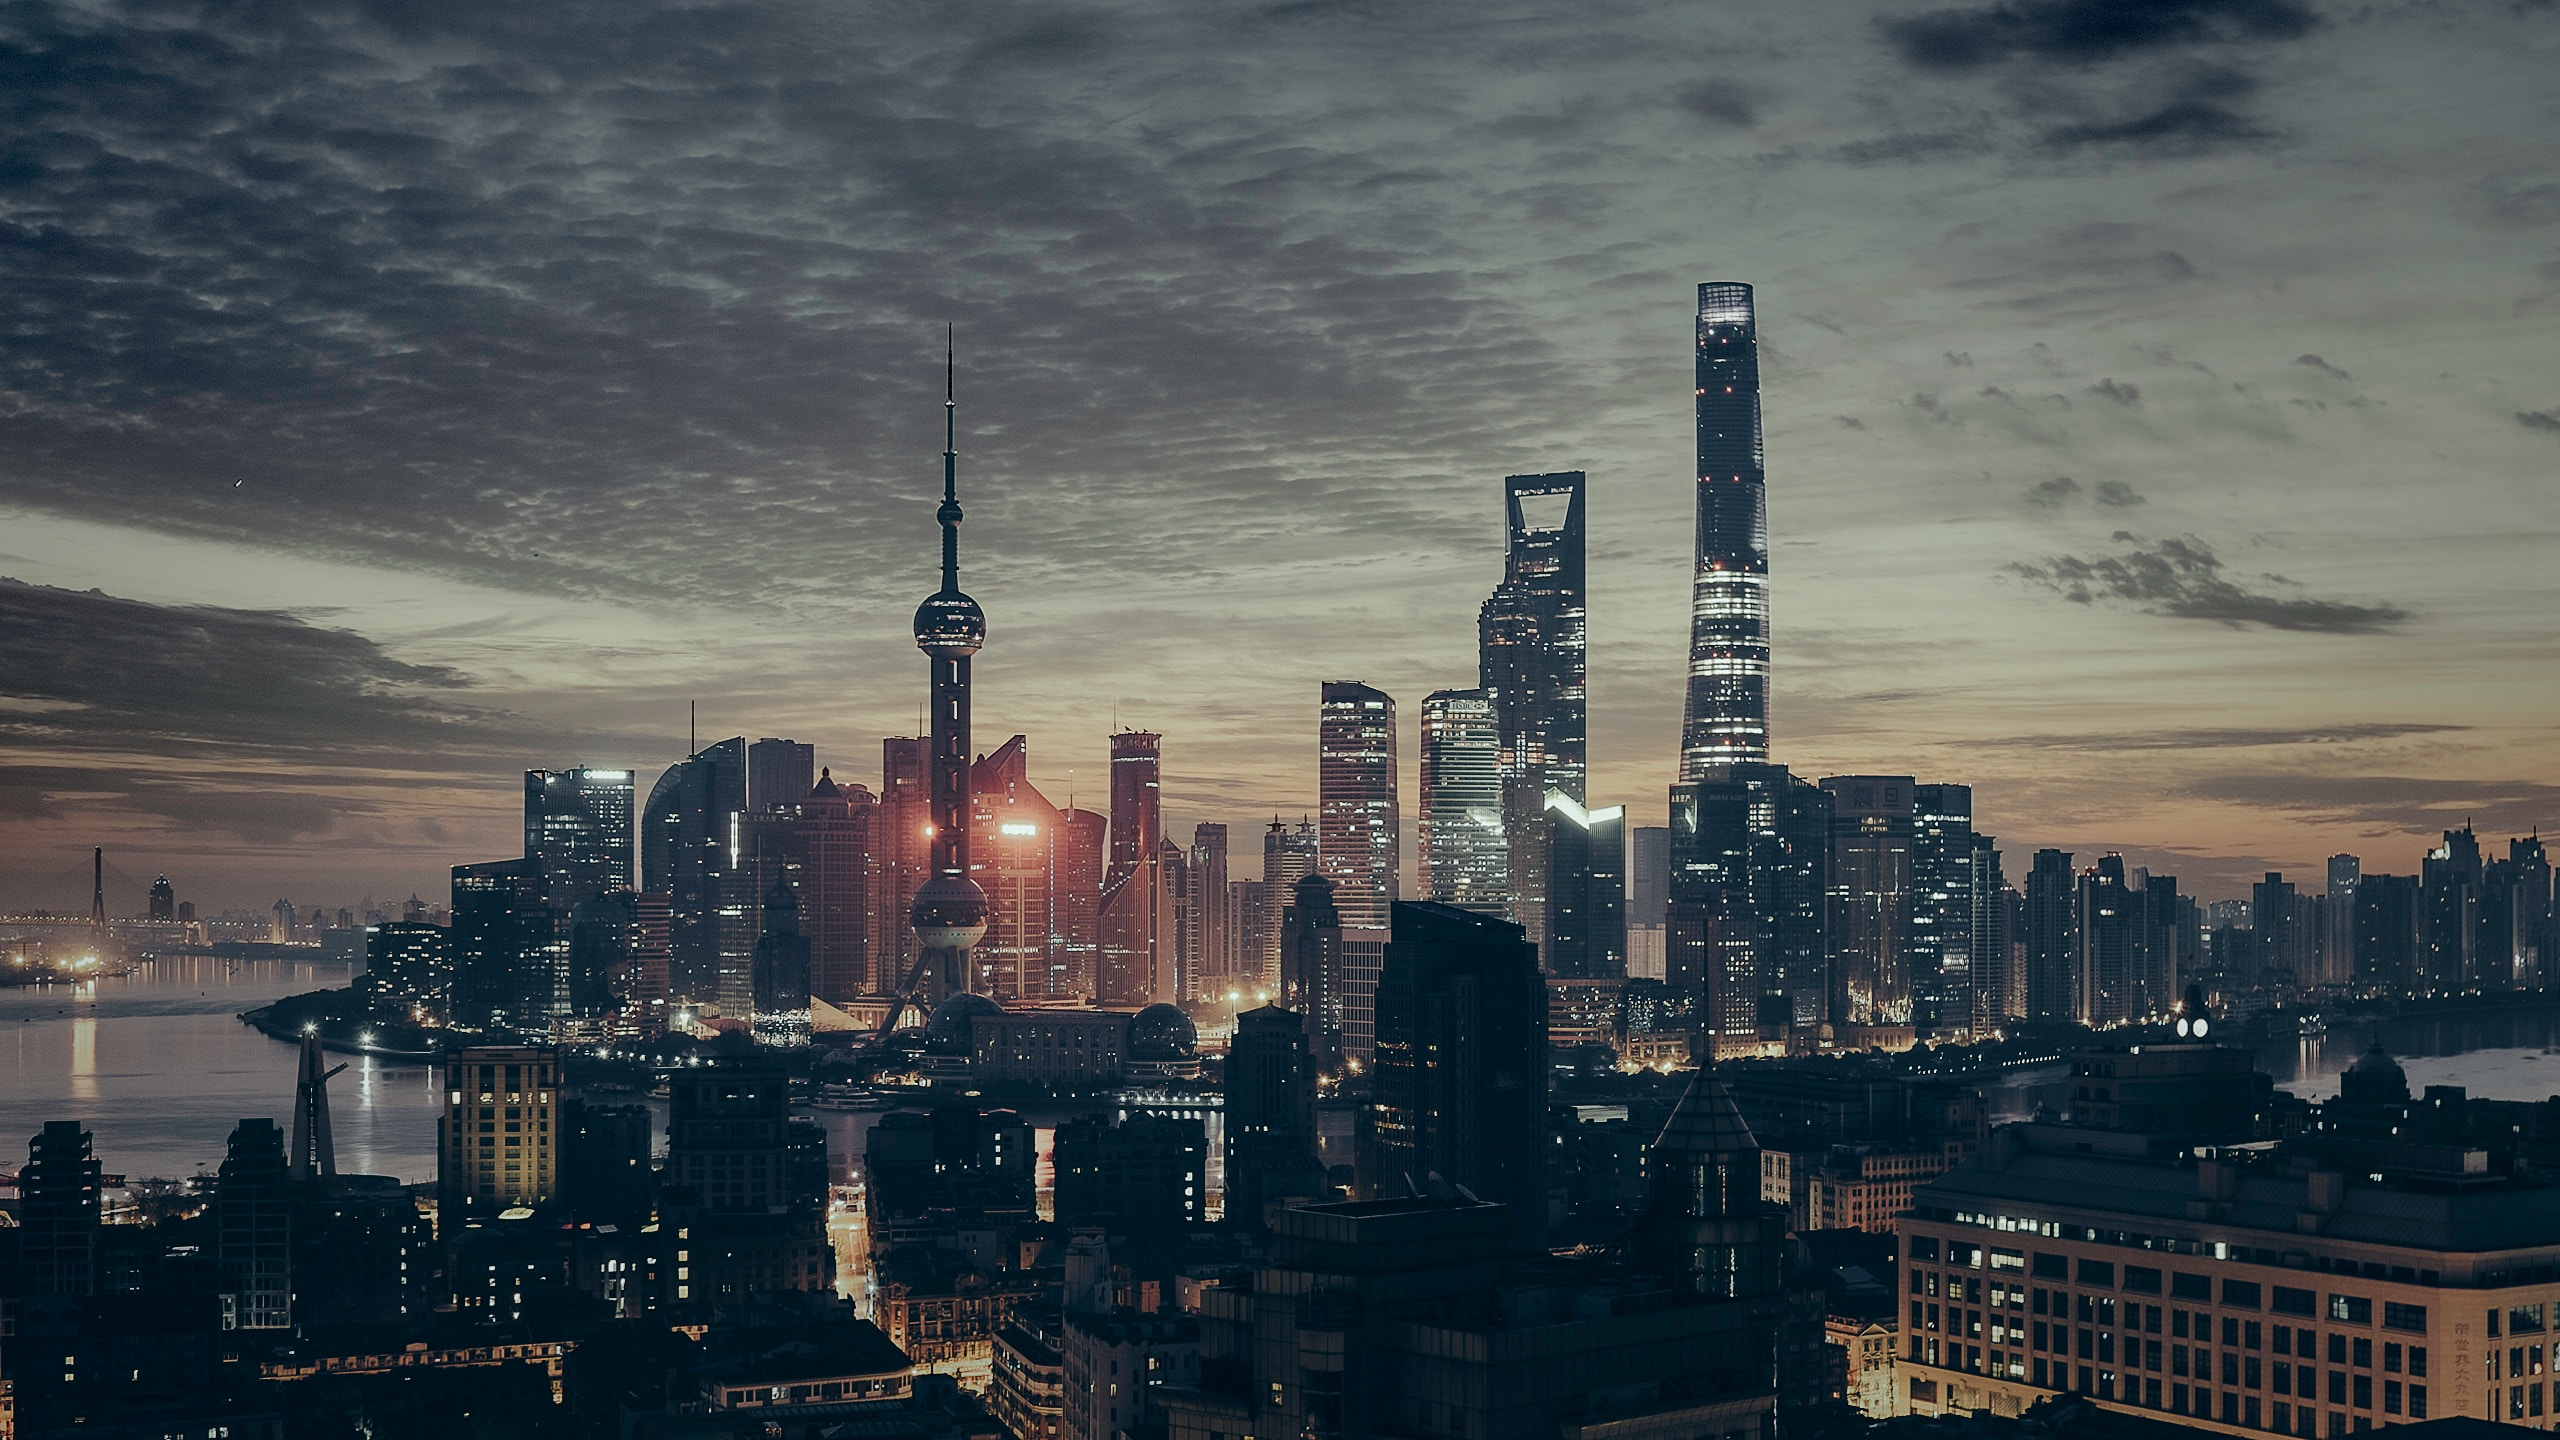
\includegraphics[scale = 0.2]{Img/china-illustration.jpg}
\end{center}
\end{figure}
\author{\Large{Marie \bsc{Chiaverini}} \Large{Baptiste  \bsc{Saclier}} \\\Large{Vadim  \bsc{Crochet}} \Large{Antoine  \bsc{Caillet}} \\\Large{Romain  \bsc{Junca}}}
\date{}
\vfill 
\end{titlepage}
\maketitle
\vspace{5.5cm}
\Large{CESI school of engineers} \hfill \Large{Tutor : Thierry \bsc{BLANC}}
\thispagestyle{empty}
\setcounter{page}{0}
\newpage

\renewcommand{\contentsname}{Table of contents}
\tableofcontents

\newpage
\renewcommand{\listfigurename}{List of figures}
\listoffigures

\newpage

\newcommand{\projectname}{ChineseTooth\xspace}
\newcommand{\moldco}{MOLD \& Co.\xspace}

\section{Introduction}

This document describes all aspects of the \projectname project which the main goal is to install IT systems around the new production line in the eco-city of Taijin.
This project includes a social and ecological aspect in order to fit to the requirements of Taijin city guidelines.

In this document, we describe what are the goals, the processes, the planning and the risk of such deployment in China.

\section{Project description}

% Description précise de tout les aspects du projet
% Quel sont les objectifs ? 
% Dans quel contexte le projet évolue il ?
% Quels sont les contraintes (Environnement, Social, Temps, Législation) ?
% Quels sont les forces et les faiblesses ?

The main goal is to install a toothbrush production line in the eco-city of Taijin in China.
Our company is workig for \moldco to make this production line a reality.

Ou main guidelines in this project is to install a production line that can produce a great amount of toothbrushes within an eco-city.
This project needs to be respectful of the surrounding environnement and social aspects of the project's stakeholders.

\subsection{Specifications}

This project has to achieve the following specifications.

The production line must contains all the required machines to automate the production of toothbrushes.
Theses machines include moulting machine, stamping machine, tufting machine, bristle cutter machine, bristle trimming machine and Packaging machine.
These machines need to be bought and connected to each other in order to build the full product.

To connect all the machines in the assembly line, the project requires also a full digital connection to an internal network.
This network group all connected machines and database servers to store monitoring informations about the production.
These informations need to represent the current production, the past production and potential errors in the production line.

The production line is fully automated throw this network and the production is regulated to produce exactly what is needed.
This automatisation brings many advantages including the environmental impact reduction, reduction of the storage requirement of finished products and 24/7 production in case of huge demand.

The informations collected need to be displayed to the employees in charge of the production line.
These informations are displayed throught an interface reading the monitoring data from the database.
A master server has to be installed in order to control all machines and to control the production flow.

Several materials are required to produce toothbrushes.
These materials are plastic, nylon, brass wire, paper box packing, plastinc hard container packaging, high frequency blister packaging and Blister card packaging.
The project must include a storage space for all these material and human resources to load the resources in the appropriate machines.

All the production line machines, storage and digital network requires engineering the organise all these components depending on the space available and the shape of the building.
Enginieering human resources are required to create, configure and install manitoring system.
Human resources may also be required to manipulate machines, connect each machine to the other and install network.

\subsection{Forces}

The forces of the project are mainly focused on the high effeciency of the production line.
This high effeciency is garanteed by the monitoring system and the automatic management of the amount of product produced on the assembly line.
This project represents a great opportunity to modernize the production of \moldco and automate the assembly line.
By automating the assembly line, \moldco gain a lot of money on storage of manufatured products and human resources.

\subsection{Weaknesses}

This project have also small weakness that may have an impact on risks
(Risk managment will be covered in the section \ref{risk-management}).

The main weakness are the important amount of advanced technologies that requires a great amount of high qualified employees in charge of the installing and maintaining the autonomous system of the assembly line.
Another weakness is the requirement of heavy and pricy machines that can represent a major part of the project's costs.

\section{Actors and Stakeholders}

% Quels sont les différents acteurs ayant un impact sur le projet ?
% Quels sont les parties prenantes et leur position dans le projet ?
% Quels sont les équipes que l'on doit mettre en place ?

\section{Project planning}

% Liste des différentes taches à éfféctuer pour atteindre les objectifs 
% Planning prévisionnel des taches
% Deadlines
% Association des équipes à chaque tache
% Quels sont les marges ? Le chemin critique ?

\begin{figure}[h]

\centering
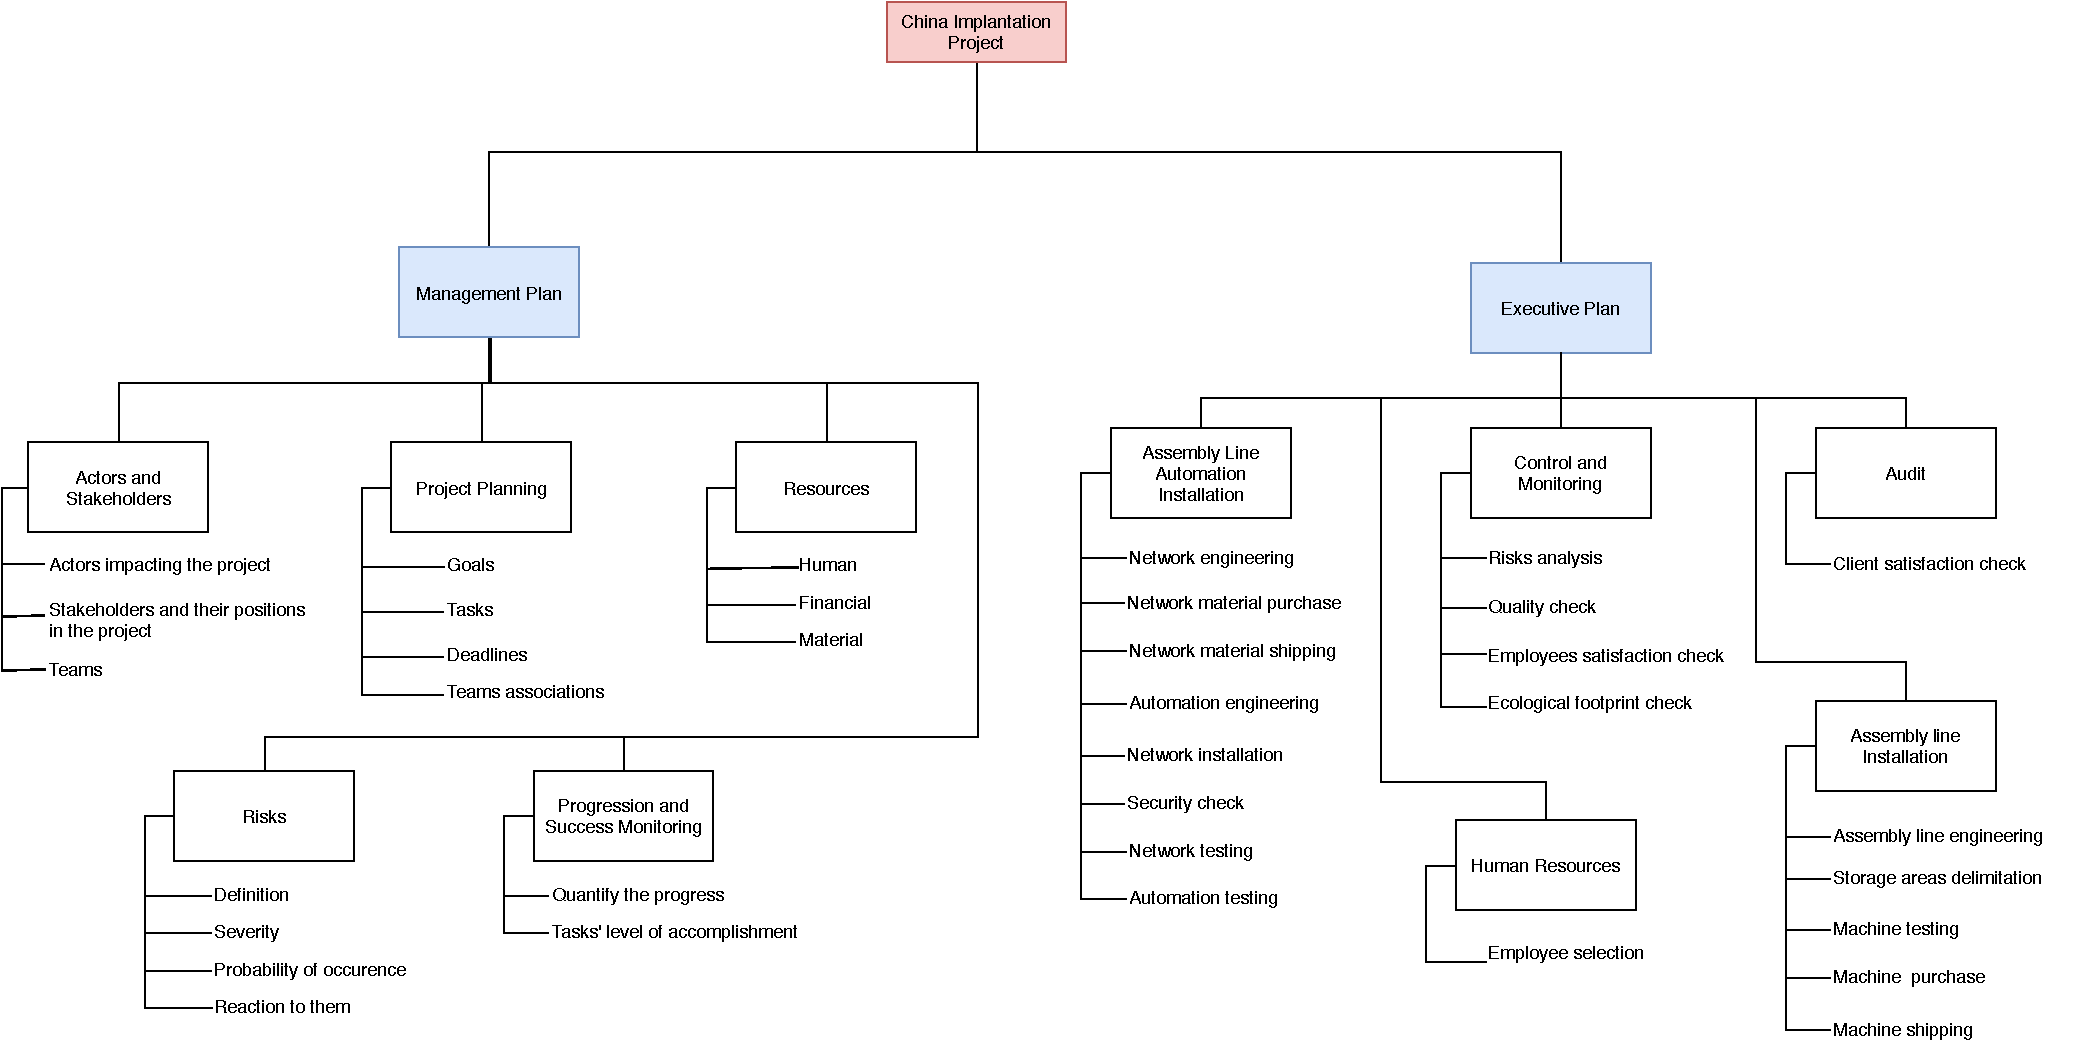
\includegraphics[scale=0.5]{Img/wbs-management-inter.pdf}
\caption{Work Breakdown Structure of the project}

\end{figure}

\subsection{Tasks}

The project is separated in many tasks that represents all steps needed to reach the goal of the project.
These tasks are separated in two categories : \emph{Managment plan} in which all the tasks represents the redaction od the management plan of the project and \emph{Executive plan} the represent the active part of the project in which the assembly line is installed.

\subsubsection{Management Plan}

The management plan is the part in which each step of the project is defined.
The management plan is defined as a frame for the project and theses tasks must be achieved before all executive task.
This part begins with a precise description of the project and goals followed by the 5 next parts.

\paragraph{Actors and Steakholders} In this parts, we must think and describe all the avtors involved in the project.
These actors are steakholders and can interact in some way with the project.
The description includes theire position, their importance and the manner that they interact with the project.
This task have also a goal of definition different teams that are required to bring this project to life.

\paragraph{Project planning} Within this task, we must think and describe all the tasks required to finish the full project, the time and resources required to achieve each task and what are task dependencies.
In this task, we must define what are deadlines and when to make debreiefing and evaluate the progression of the project.

\paragraph{Resources} In this part of the project, we must identify and write the required resources to achieve each task defined in the \emph{Project planning} part.
These resources include : human resources, financial resources and material resources.

\paragraph{Risks} In this task, we must define the primary risks that can occur during the project and how to reduce the side effect of each risk.
Each risk have a severity and prbabilty rate that represent the criticity of it.
Higher the criticity is, important the risk must be and planned with caution.

\paragraph{Progression and success monitoring} Finally, in the progression monitoring we must identify what indicator can represent the progression or the success of each task and the whole project.
These indicator will be used all along the project to define it's progression and if some task are taking late.

\subsubsection{Executive Plan}

The executive plan indicates all actions done after the work on the management plan. 
This category includes the installation of the assembly line and its automation, but also its control and monitoring, in addition of the human resources and an audit of the client.

\paragraph{Assembly Line Installation} This part aims to identify the processes brought by the installation of the assembly line. 
After an assembly line engineering, in which we study the building disposal, where and how the machines will connect with themselves, we also
study the place for the storage areas. 
We then test the machines after their purchase and their shipping. 

\paragraph{Assembly Line Automation installation} This part is about the automation of the assembly line, which includes a network engineering (the study of the disposal of the network in the building), the purchase
of the material for this network (routers, switches, etc.) and their shipping to the building, before their installation and test. 
We also study the automation of the machines, how it will work, and how to put it in place, with also a testing session and a security check.

\paragraph{Human Resources} The human resources part identify the employee selection process. Those employees 
must be fit to the required tasks of the executive plan. To the study of the building and other engineering around the machines to the 
installation of the automation of those machines, and their control and monitoring. 

\paragraph{Control and Monitoring} After the installation of the machines and their automation set, we must control and regulate them.
This includes the risks analysis process, which means a constant control and verification of the assumed risks but also an answer plan in the case of a crisis situation. 
We also check on the quality of the machines, their cleanliness and their working order, but also on the employee's satisfaction as we want to be sure they
work in an environnement as comfortable as possible. 
In the same way, we want a constant control of the ecological footprint of the building to respect our environmental engagements.   

\paragraph{Audit} Finally, this task is required to retreive some feedback from the client.
These feedback can lead to an improvement process and can be added to our quality pipeline in order to continuously improve our practices.



\section{Required resources}

% Quels sont les moyens humains nécéssaires ?
    % Equipes
    % Formations
    % Nombres d'heures
% Quels sont les moyens financiers requis ?
% Quels sont les moyens materiel requis ?

\section{Risks management}
\label{risk-management}

% Quels sont les risques encourus durant le projet ?
% Quel est la sévérité, la probabilité d'apparition ?
% Quel opérations mettre en place pour les risques les plus graves ?

\section{Indicators of progression and success}

% Comment peut on quantifier l'avancement du projet ?
% Quel est l'indicateur permettant de définir qu'une tache est accomplie et valide ?

\section{Conclusion}



\end{document}

